\documentclass[crop, tikz]{standalone}

\usepackage[utf8]{inputenc}
% 'crop' is the default for v1.0, before it was 'preview'
%\usetikzlibrary{...}% tikz package already loaded by 'tikz' option

\usetikzlibrary{arrows}
\usetikzlibrary{decorations.markings}
\usetikzlibrary{patterns}
\usetikzlibrary{calc}

\begin{document}
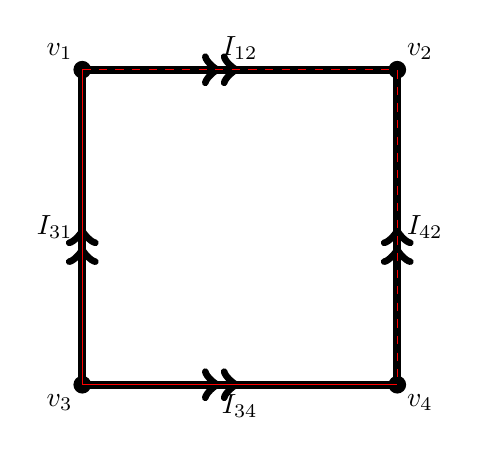
\begin{tikzpicture}[]

	\def\L{4} %period cell size
	\def\vThick{3} %vertex dot size in pt
	\def\lThick{3} %line width in pt
	%vertex locations
	\coordinate (v1) at (0,\L);
	\coordinate (v2) at (\L,\L);
	\coordinate (v3) at (0,0);
	\coordinate (v4) at (\L,0);
	%vertex rendering
	\filldraw[black] (v1) circle (\vThick pt) node[anchor=south east] {$v_1$};
	\filldraw[black] (v2) circle (\vThick pt) node[anchor=south west] {$v_2$};
	\filldraw[black] (v3) circle (\vThick pt) node[anchor=north east] {$v_3$};
	\filldraw[black] (v4) circle (\vThick pt) node[anchor=north west] {$v_4$};

	%edge drawings
	\begin{scope}[decoration={markings, mark=at position 0.5 with {\arrow{>>}}}]
		\draw[black, line width=\lThick pt, postaction=decorate] (v1) -- (v2);
		\node[anchor=south] at ($(v1)!0.50!(v2)$) {$I_{12}$};
		\draw[black, line width=\lThick pt, postaction=decorate] (v3) -- (v1);
		\node[anchor=east] at ($(v3)!0.50!(v1)$) {$I_{31}$};
		\draw[black, line width=\lThick pt, postaction=decorate] (v3) -- (v4);
		\node[anchor=north] at ($(v3)!0.50!(v4)$) {$I_{34}$};
		\draw[black, line width=\lThick pt, postaction=decorate] (v4) -- (v2);
		\node[anchor=west] at ($(v4)!0.50!(v2)$) {$I_{42}$};
	\end{scope}

	%domain boundaries for clarity
	\draw[red] (v1) -- (v3) -- (v4);
	\draw[red, dashed] (v1) -- (v2) -- (v4);

\end{tikzpicture}
\end{document}